\documentclass{article}
\usepackage[utf8]{inputenc}
\usepackage{xcolor}
\usepackage{amsmath}
\usepackage{url}
\usepackage{graphicx}
\usepackage{natbib}
\usepackage{algorithm} 
\usepackage{algpseudocode} 
\usepackage{multirow}
\usepackage{makecell}
\usepackage{subcaption}
\usepackage{eurosym}
\usepackage{url}
\usepackage{amssymb}
\usepackage{adjustbox}
\usepackage{caption}


\bibliographystyle{abbrvnat}
\setcitestyle{authoryear,open={(},close={)}}
\usepackage[a4paper,width=150mm,top=20mm,bottom=25mm]{geometry}
%%%%%%%%%%%%%%%%%%%%%%%%%%%%%%%%%%%%%%%%%%%%%%%%%%%%%%%%%%%%%%%%%%

\title{
{Operational Research: Theory and Applications}\par
\vspace{12pt}

\includegraphics[width=50mm]{report-2/fig/logo.png}\par
{ Shop ordering problem - Group 16} \par
}
\vspace{5pt}
\date{ ICT for Smart Societies 2019-2020}
\author{Andrea Avignone - 279954\\
		Tommaso Carluccio - 276909\\
		Vincenzo Madaghiele - 277028\\}
\begin{document}
\maketitle
\begin{abstract}
\noindent
The purpose of this project is the creation of a mathematical model to describe the multi-period ordering planning of a generic store. The LP formulation is implemented in a Python environment, exploiting the PuLP library. The analysis on the case study is performed considering both an exact and a heuristic solution. After some instances generation, computational results are provided to offer a complete overview of the project and its functionalities.
\end{abstract}
\section{Introduction}
The aim of this model is to optimize the classical inventory problem, organizing the ordering system to maximize the profit. The considered scenario refers to a shop selling different products according to the evolution of the demand over a generic time period. 
The basic unit of time for the simulation, referred as time step in the following, can be associated to a day. The simulation runs for a time period which is always a multiple of the time steps. \par
At each time step, an order can be made from a set of suppliers, characterized by different prices and discounts. For example, a supplier could not have some of the requested products. The order is not immediate, it takes an established amount of time steps to arrive. Its cost is the consequence of three contributions: a fixed cost necessary to start the order from a certain supplier, a unitary cost for each purchased item and a discount dependent on the total quantity purchased from the supplier (independently by the type of product) following a step-wise function. At the beginning of each day the shop inventory is updated adding the orders arrived at that time step and subtracting the items sold the day before. \par 
In addition, the model takes into consideration an holding cost for stock products and an extra cost proportional to the unsatisfied demand. It is worth noticing that, while the extra cost due to the unsatisfied demand only holds when the demand is not met, the holding cost is applied whenever an item is stored in the inventory, even if it is yet to be sold. The shop also sets a selling price for each product. At any period, the minimum between the available inventory quantity and the demand for a specific item is sold.
Furthermore, the optimization begins from an initial condition of the inventory and from a set of orders supposedly made before the starting point of the simulation, referred as pre-order in the paper. They are expected to arrive along the simulation time period, exactly as the adjustable orders made during the optimization procedure.\par
The effects of different instances will be analyzed, showing how the designed system responds according to the considered situation. Besides all of the deterministic parameters, the optimization strategy is necessarily based on the expected demand at each time step, which instead should be read as an estimation computed by the shop owner. The importance of this aspect is further explored in the following sections to investigate its weight in the general system.\par
Along with the optimal model, an Heuristic one is provided, which exploits the Greedy Approximate Dynamic Programming approach. This procedure is a compromise between the solution efficiency and the time complexity of the exact model. This is achieved by reducing the solution space of the optimal one, by solving many smaller LP problems corresponding to a single time step and by introducing some heuristic constraints.

%%%%%%%%%%%%%%%%%%%%%%%%%%%%%%%%%%%%%%%%%%%%%%%%%%%%%%%%%%%%%%%%%
\section{Literature Review}
The implemented formulation could be extended to several applications, including more specific conditions. Taking optimal decisions is an important step to optimize costs for any sort of activity. \cite{Papageorgiou2001}, for example, showed this aspect in the Pharmaceutical Industries. However, finding the best trade-off to meet the demand is not always straightforward. \cite{James1999} treated inventory constraints for the multi-period organization, given the demand evolution. Therefore, the supply chain is a crucial focus of logistics to maximize the profit, avoiding to exceed a competitive selling price.  Coordination mechanism to reduce costs is considered by \cite{Khouj2003}. Moreover, the starting point of the proposed model is actually an evolution of the classical transportation problem. It is necessary to choose the most convenient facility to order from. The double nature of the Traveling Purchaser Problem is analyzed by \cite{Maner2016}. Uniformly, \cite{Aissa2007} presented an optimization for order planning and supplier selection. \par
Some interesting features could be joined to have a more realistic and useful model, obviously increasing its complexity and time of performance. Among them, probably the most relevant ones are: the capacity of both suppliers and inventory, the possibility of damaged goods, the prices variation along the time horizon, the introduction of perishable goods. The case in which ordered products are not perfect in quality is treated by \cite{Rezae2018}. In \cite{Mousavi2014} paper, the minimization of the total inventory cost includes also considerations about inflation, besides costs of holding, purchasing and shortage. \par
For its already mentioned importance, during the past years the multi-period inventory scheduling has been involved in different studies, trying to optimize the related algorithm despite the increasing complexity. The importance of supplier selection in a lot sizing problem was presented by \cite{Basnet2005}. Similarly, \cite{Vargas2009} proposed an algorithm based on the popular Wagner–Whitin model. \par
In this paper, an important role concerns suppliers discounts. \cite{Khosr2016} optimized a dynamic lot sizing problem with a formulation of the model based on the discount of purchasing cost. \cite{Calle1977} used a MIP model to find the optimal planning, exploiting binary decision variables. \par
Since an exact approach is not often suitable for the necessary simplifications, heuristic strategies are usually preferred. \cite{Wagner2004} handled multiple products in a single facility with limited capacity through local search. A common heuristic approach for this kind of problem is the Approximate Dynamic Programming (ADP), which is generally applied to problems modeled using optimal Dynamic Programming (DP). In most cases the two approaches are mixed to obtain high performance using an heuristic method, but in this paper only the pure greedy ADP is implemented, mainly because the optimal solution is modeled as a LP problem, not a DP. The heuristic method implemented in this report is based on the solution of many smaller LP problems, differently from the ones typically found in the literature, which are usually based on a modification of a DP model. The main concepts implemented in this heuristic solution, although with all the aforementioned differences, are based on the models formulated by \cite{Cimen2013} and \cite{Meiss2018}. 
\par
\newpage
\section{Mathematical Model}\label{sec:mathModel}
In this section, the mathematical model is presented. All the parameters used for the model are displayed in Table \ref{tab:parameters}, together with the chosen fundamental and auxiliary decision variables. The notation will be enhanced in the model definition, while the values of parameters should be the key for effective demonstrations according to their influence. \begin{table} [H]
    \centering
    \begin{subtable}[c]{\textwidth}
        \centering
	    \begin{tabular}{|c|c|} 
		\hline
		\textbf{Notation} & \textbf{Meaning}  \\
		\hline
		$\Theta$ & Set of products\\
		$\Lambda$ & Set of suppliers\\
		$T$ & Time period \\
		$C_f^j$ & Fixed cost for supplier j \\
		$e^i$ & Extra cost due to unsatisfied demand\\
		$c^{i,j}$ & Cost of one item i from supplier j\\
		$h^i$ & Unitary holding cost for product i\\
		$I^i_0$ & Initial inventory of product i\\
		$D^i_t$ & Demand of product i at time $t$ \\
		$p_i$ & Selling price of product i\\
		$P_t^i$ & Pre-order of product i before t=0\\
		$T^i$ & Time needed for product i to arrive \\ 
		$thr^j_{l}$ & Threshold of discount batch $l$ of supplier $j$\\ 
		$d^j_l$ & Percentage discount applied by supplier $j$ for batch $l$\\
		\hline
		\end{tabular}
        \caption{Parameters}
        \vspace{5mm}
    \end{subtable}
	
    \begin{subtable}[c]{\textwidth}
        \centering
	    \begin{tabular}{|c|c|} 
		\hline
		\textbf{Notation} & \textbf{Meaning} \\
		\hline
		$I^i_t$ & Inventory of product i at time $t$ \\
		$O^{i,j}_t$ & Amount of product i ordered from supplier j at time $t$\\ \hline
		$b^i_t$ & Unsatisfied demand of product i at time $t$ \\
		$y^j_t$ & Binary variable equal to 1 if order from supplier j at time t is made\\
		$s^i_t$ & Implemented variable to linearize $min[D^i_t, I^i_t]$\\
		$w^j_{l,t}$ & Implemented binary variable to linearize the discount function \\
		$\delta^j_{l,t}$ & Implemented binary variable to linearize the discount function \\
		$totD^j_t$ & Total discount applied by supplier $j$ at time $t$\\
	    \hline
	    \end{tabular}
        \caption{Decision variables} 
        \vspace{5mm}
        \end{subtable}  
        \caption{List of problem parameters and decision variables}
        \label{tab:parameters}
\end{table}
The objective function concerns the maximization of the profit. Earnings are generated by selling the products according to the daily demand for each one. Given a selling price, clearly the main focus moves to the minimization of the transportation and the inventory costs. In fact, the core of the ordering strategy consists in the selection of the right amount of products to be purchased from each single supplier, observing some constraints.\\ The objective function formula is shown in Equation (1-\ref{EQPB:objts}). As it can be seen, it is based on the subtraction of all the cost sources from the selling revenue and the eventual discount performed by the suppliers. \par
In a more realistic environment, the selling price should be the outcome of some marketing evaluations, accordingly to the actual cost of goods. Therefore, an other decision variable should be implemented, dedicated to this purpose; but this kind of evaluation is out of the main focus of the paper. Optimizing the selling prices would be shallow without any proper market analysis. Indeed, prices are set independently, assuming the suited considerations were already made. Nevertheless, the unitary costs $c^{i,j}$ of provisioning by suppliers are generated in order to be consistent with the pre-defined selling prices. \par
Each supplier offers a discount based on the total number of items requested by an order, regardless of the type of the item. The discount is calculated as a percentage on the fixed cost, explainable as a reduction on the delivery cost. This should be read as a stimulus to order more products from the same supplier. It is modelled using a step function with a qualitative behaviour similar to the one depicted in Figure \ref{fig:discount}. In other words, if an order is included in one of the available ranges, it will be affected by the corresponding discount. The distribution of the cost reduction is different for each supplier, both in terms of necessary amount of items (width of the step) and expected discount (height of the step). The result is a diversified set of possible scenarios and preferences.
The model is summarized as follows:

\begin{eqnarray}
\max && \sum_{i=0}^\Theta \sum_{t=0}^T p_i  s_t^i - \sum_{j=0}^\Lambda \sum_{t=0}^T Cf^j  y_t^j - \sum_{i=0}^\Theta \sum_{j=0}^\Lambda \sum_{t=0}^T c^{i,j} O_t^{i,j} -
\sum_{i=0}^\Theta \sum_{t=0}^T h^i I_t^i-  \\ & &
\sum_{i=0}^\Theta \sum_{t=0}^T e^i b_t^i +
\sum_{j \in {\Lambda}_i} \sum_{t=0}^T totD_t^j
\label{EQPB:objts} \\
s.t. && I_t^i=I_{t-1}^i+O_{t-T^i}^i - D_{t-1}^i \qquad t-T^i \geq 0, \forall i \in \Theta, t \in T \label{EQPB:inventory} \\
&& I_t^i=I_{t-1}^i+P_{t-T^i}^i - D_{t-1}^i \qquad t-T^i < 0, \forall i \in \Theta,  t \in T \label{EQPB:inventory_preorder} \\
&& I_t^i=I_{0}^i \qquad \forall i \in \Theta,\; t=0 \label{EQPB:init_inventory} \\
&& \sum_{j=0}^\Lambda O_t^{i,j} \leq M y_t^i \qquad \forall i \in \Theta,  \forall t  \in T\\
&& b_t^{i} \geq D_{t}^i - I_t^i, \qquad \forall i \in \Theta,  \forall t  \in T  \label{EQPB:b}\\
&& s_t^i \leq I_t^i, \qquad \forall i \in \Theta,  \forall t  \in T\\
&& s_t^i \leq D_t^i, \qquad \forall i \in \Theta,  \forall t  \in T\\
&& \sum_{i=0}^\Theta O^{i,j}_t \leq thr^j_l + M (1 - w^j_{l,t}), \qquad \forall j  \in \Lambda, \forall t  \in T, l=0\\
&& \sum_{i=0}^\Theta O^{i,j}_t \geq thr^j_l + m \ w^j_{l,t}, \qquad \forall j \in \Lambda, \forall t  \in T, l=0\\
&& \sum_{i=0}^\Theta O^{i,j}_t \leq (thr^j_{l-1}+1) + M \ \delta^j_{l,t} + M \ w^j_{l,t}, \qquad \forall j \in \Lambda, \forall t  \in T, l=1,2\\
&& \sum_{i=0}^\Theta O^{i,j}_t \geq thr^j_l - M (1-\delta^j_{l,t}) - M \ w^j_{l,t}, \qquad \forall j \in \Lambda, \forall t  \in T, l=1,2\\
&& \sum_{i=0}^\Theta O^{i,j}_t \geq (thr^j_{l-1}+1) - M (1 - w^j_{l,t}), \qquad \forall j \in \Lambda, \forall t  \in T,l=1,2\\
&& \sum_{i=0}^\Theta O^{i,j}_t \leq thr^j_l + M (1- w^j_{l,t}), \qquad \forall j \in \Lambda, \forall t  \in T, l=1,2\\
&& \sum_{i=0}^\Theta O^{i,j}_t \leq thr^j_l + M \ w^j_{l,t}, \qquad \forall j \in \Lambda, \forall t  \in T, l=3\\
&& \sum_{i=0}^\Theta O^{i,j}_t \leq thr^j_l + m (1 - w^j_{l,t}), \qquad \forall j \in \Lambda, \forall t  \in T, l=3\\
&& totD^j_t = f^j\sum_{l=0}^3 d^j_l w^j_{l,t}, \qquad \forall j \in \Lambda, \forall t  \in T\\
&& I_t^i \geq 0 \qquad \forall i \in \Theta,\; \forall t \in T \label{EQPB:general_inventory} \\
&& y_t^j =\{0,1\}, \qquad \forall j \in \Lambda, \forall t \in T \label{EQPB:supplier}\\
&& O_t^{i,j} \geq 0, \qquad \forall i \in \Theta, \forall j \in \Lambda, \forall t  \in T \label{EQPB:amount}\\
&& b_t^{i} \geq 0, \qquad \forall i \in \Theta,  \forall t  \in T \label{EQPB:b0}\\
&& s_t^i \geq 0, \qquad \forall i \in \Theta,  \forall t  \in T\\
&& w_{l,t}^j = \{0,1\} \qquad \forall j \in \Lambda, t \in T, l=1,2,3\\
&& \delta_{l,t}^j=\{0,1\} \qquad \forall j \in \Lambda, t \in T, l=1,2,3\\
&& totD_t^j \in \mathbb{R}
\end{eqnarray}
\noindent
\newpage
The constraints (3) and (4) are related to the inventory balance. The amount of product $i$ at time $t$ is the sum of the residual inventory at $t-1$ plus the order realized $T^i$ steps before, subtracting the demand for the product at time $t-1$. However, a distinction needs to be stressed if the condition involves an hypothetical order made before the origin of the time horizon. Obviously, the optimization should not involve the situation before $t=0$. In this scenario, a pre-order (with the possibility to be set to 0) is considered: it is the list of products ordered before the optimizing phase. The statement (5) sets, instead, the condition for the initial inventory of the warehouse. This is a main feature, since the model aspires to be the solution for an inventory optimization, knowing its starting point. Feasibility is ensured by (19), imposing the inventory to be always equal or greater than zero. \par
The binary variable defined in constraint (20), as any basic transportation problem, indicates if the plant $j$ will be open at time $t$ with a fixed cost. This condition is directly linked to the logical constraint (6) where $M$ is a large enough number, knowing by (21) that the order must not be negative. This variable is clearly related to the unitary cost of each order. \par
Statements (7) and (22) concern the unsatisfied demand cost, proportional to the level of dissatisfaction ($e^i$ is the unitary cost) or set to zero if the demand is completely met. \\ Another relevant aspect is related to the holding cost of each item, as shown in the objective function. At every time instant $t$, it is proportional to the quantity of each item in the inventory, read as warehouse maintenance costs. Simulations will show the impact of this value in the distribution of performed orders along the time. Instead, equations (8), (9) and (23) describe the auxiliary decision variable which takes the value of the minimum between the inventory and the demand for each product at each time step. It corresponds to the quantity of product which is sold at time $t$. \par
The discount is described by the non-linear equation (27), and depicted in Figure \ref{fig:discount}. 

\begin{equation}
    u_t^j\Big(\sum^{\Theta}_{i=0}O_t^{i,j}\Big)=
    \begin{cases}
    0 & \textit{if} \quad 0 <\sum_{i=0}^{\Theta}O_t^{i,j}<thr^j_0\\
    d^j_0 & \textit{if} \quad (thr^j_0+1)<\sum_{i=0}^{\Theta}O_t^{i,j}<thr^j_1\\
    d^j_1 & \textit{if} \quad (thr^j_1+1)<\sum_{i=0}^{\Theta}O_t^{i,j}<thr^j_2\\
    d^j_2 & \textit{if} \quad (thr^j_2+1)<\sum_{i=0}^{\Theta}O_t^{i,j}
    \end {cases}
\end{equation}

The not straightforward linearization of the discount function is shown in equations (10)-(17). It is applied by supplier $j$ at time $t$, given the total quantity of items that have been ordered from it. The central and generic blocks are defined by statements (12)-(15), while the peculiar ones are described by (10)-(11) for the case with zero discount, and (16)-(17) for the maximum (with M a large enough number and m a strong negative number). The crucial aspect is the determination of the belonging block, according to different thresholds. For this purpose, binary variables (24) and (25) are implemented. For each block, the corresponding percentage of discount is introduced by the integer parameter $d_t^j$. Finally, the total discount on shipping cost is obtained by (18), avoiding the unfeasible overlapping of discounts.
Clearly, each supplier presents different thresholds and percentage values to be competitive. 

\begin{figure}[!ht]
    \centering
    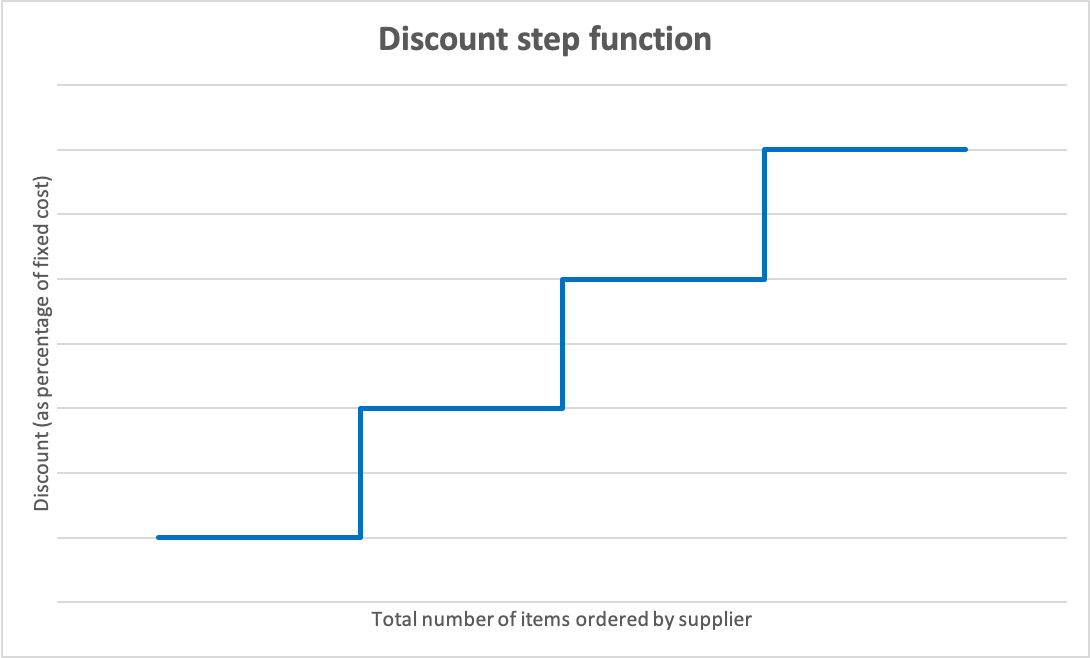
\includegraphics[width=0.7\textwidth]{report-2/fig/discount.png}
    \caption{Discount function qualitative behaviour \label{fig:discount}}
\end{figure}
\section{Instance generation}\label{sec:instance}
In order to run a simulation of the model, an instance of the problem must be introduced. In Table \ref{tab:description}, a generic instance is proposed, following some reasonable criteria to generate an appropriate environment. It is the actual description of the shop features, considering the initial condition and maintenance costs for each specific item (Table 2a). Ten products are taken into account to be consistent, varying in both costs and arrival time. \par
For the suppliers definition, Table 2b is used. The three considered suppliers present a fixed cost for the order initialization and a specific unitary cost for each available product. Obviously, the final strategy adopted by the model is strictly related to all the values. \par
These parameters are mainly used in the comparison between the exact solution and heuristic one. 
All the just described values are chosen in order to be as realistic as possible. For example, the same boundary values are assigned to the demand, the initial inventory and the pre-order. In a realistic scenario, in fact, the quantity of items in the inventory should be proportioned to the expected demand. Therefore, this main instance is the core for any complete check on model capabilities. Nevertheless, parameters can be freely tuned to meet all simulation needs, depending on the desired kind of activity. In Section \ref{subsec:computational_results_exact}, instead, starting from this structure, several instances are generated to analyze different behaviours, studying the most important cases. For this purpose, some \textit{ad hoc} instances will be considered to stress the main peculiarities of the project.
\begin{table}[H]
\vspace{20pt}
    \centering
    \begin{subtable}[c]{\textwidth}
    \centering
    \begin{adjustbox}{center}  
    \begin{tabular}{|c|c|c|c|c|c|}
    \hline
     & \makecell{\textbf{\makecell{Initial \\Inventory}}} & \makecell{\textbf{Selling Price}\\$[euros]$} & \makecell{\textbf{Arrival time}\\$[days]$} & \makecell{\textbf{Holding Cost} \\$[euros]$} & \makecell{\textbf{Extra Cost} \\$[euros]$} \\
    \hline
    \textbf{Product 1} & 55 & 35 & 5 & 5 & 5\\
    \hline
    \textbf{Product 2} & 72 & 27 & 2 & 3 & 5\\
    \hline
    \textbf{Product 3} & 60 & 15 & 3 & 6 & 5\\
    \hline
    \textbf{Product 4} & 54 & 22 & 5 & 6 & 2\\
    \hline
    \textbf{Product 5} & 42 & 33 & 4 & 5 & 3\\
    \hline
    \textbf{Product 6} & 65 & 34 & 4 & 4 & 4\\
    \hline
    \textbf{Product 7} & 44 & 33 & 1 & 2 & 3\\
    \hline
    \textbf{Product 8} & 89 & 36 & 5 & 5 & 4\\
    \hline
    \textbf{Product 9} & 96 & 36 & 4 & 4 & 2\\
    \hline
    \textbf{Product 10} & 38 & 27 & 5 & 6 & 3\\
    \hline
    \end{tabular}
    \end{adjustbox}
    \caption{Shop parameters for inventory}
    \vspace{20pt}
    
    \end{subtable}
    
    \begin{subtable}[c]{\textwidth}
        \centering
    \begin{tabular}{|c|c|c|c|c|}
    \hline
    & \makecell{\textbf{Fixed cost}} & \makecell{\textbf{Unitary costs of products} \\$[euros]$}  \\
    \hline
    \textbf{Supplier 1} & 115 & 9 19 14 3 17 8 32 29 31 21  \\
    \hline
    \textbf{Supplier 2} & 187 & 25 26 4 4 32 2 25 28 1 23  \\
    \hline
    \textbf{Supplier 3} & 116 & 1 13 11 7 28 2 15 29 32 18 \\
    \hline
    \end{tabular}
    \caption{Suppliers parameters}
    \end{subtable}
    \caption{Generic instance for a pseudo-real model }
    \label{tab:description}
    \vspace{20pt}
\end{table}

Also the discount functions of each supplier should be defined following balanced rules. In fact, thresholds for the discount are chosen randomly between some defined boundaries for every section of the function. In this way, suppliers differ for both the width of blocks (quantity of items) and the associated discount on the fixed cost. The block is chosen between zero and the first threshold for the first step and between the chosen value of the previous step and the next threshold for the subsequent steps. The same approach is used to choose the discount percentage. All ranges are summarized in Table \ref{tab:discounts}.
Since each supplier makes its own decision for each block based on the one before, in Table \ref{subtab:limits} columns are mainly characterized by the specified upper limit, in charge of ensuring a competitive market. Instead, the last upper limit of the fourth block (referred to the amount range) in Table \ref{subtab: supplier_discounts} should be read as a capacity constraint imposed by the supplier itself. It is actually impossible to have an infinite final block in terms of realistic products amount. Even though the boundary is necessary, it must be carefully selected. Otherwise, a large - but still reasonable - order might not belong to any block. Imposing a remarkable final limit (compared to the problem specifics) avoids this kind of issues.
\newline

\begin{table}[H]
    \centering
    \begin{subtable}[c]{\textwidth}
        \centering
    \begin{tabular}{|c|c|c|c|c|}
    \hline
    & \makecell{\textbf{First Block}\\\textbf{(Limits)}}  & \makecell{\textbf{Second Block}\\\textbf{(Limits)}} & \makecell{\textbf{Third Block}\\\textbf{(Limits)}} & \makecell{\textbf{Fourth Block}\\\textbf{(Limits)}}\\
    \hline
    \textbf{Range} & 1-20 & 21-100 & 101-150 & 151-10000 \\
    \hline
    \textbf{Discount} & 0\% & 1-30\% & 31-50\% & 51-70\% \\
    \hline
    \end{tabular}
    \caption{Discount boundaries}
    \label{subtab:limits}
    \vspace{5mm}
    \end{subtable}

    \begin{subtable}[c]{\textwidth}
        \centering
    \begin{tabular}{|c|c|c|c|c|}
    \hline
    & \textbf{First Block} & \textbf{Second Block} & \textbf{Third Block} & \textbf{Fourth Block}\\
    \hline
    \textbf{Supplier 1} & 1-8 & 9-53 & 54-83 & 84-3668 \\
    \textbf{Discount} & 0\% & 10\% & 12\% & 39\% \\
    \hline
    \textbf{Supplier 2} & 1-18 & 19-31 & 32-55 & 56-4912 \\
    \textbf{Discount} & 0\% & 24\% & 35\% & 68\% \\
    \hline
    \textbf{Supplier 3} & 1-14 & 15-79 & 80-104 & 105-5075 \\
    \textbf{Discount} & 0\% & 19\% & 48\% & 64\% \\
    \hline
    \end{tabular}
    \caption{Suppliers discounts}
    \label{subtab: supplier_discounts}
    \end{subtable}
    \caption{Generation of discount functions }
    \label{tab:discounts}
\end{table}
\subsection{Computational Results}\label{subsec:computational_results_exact}
The model is tested in different scenarios in order to stress its most peculiar features. The validity of the project is proved both through some borderline cases and a more realistic instance. Simulations are performed in a Python environment, using CBC solver.  \newline
Initially, the solution is the response to the demand evolution of Table \ref{tab:dem_ev}, randomly generated. At each step, a new parameter is included, providing a smoother study of the system capabilities.
\newline

\begin{table}[H]
    \centering
    \begin{tabular}{|c|c|c|c|c|c|c|c|}
    \hline
    & \textbf{\textit{t=0}} & \textbf{\textit{t=1}} & \textbf{\textit{t=2}} & \textbf{\textit{t=3}} & \textbf{\textit{t=4}} & \textbf{\textit{t=5}} & \textbf{\textit{t=6}}\\
    \hline
    \textbf{Product 1} & 59 & 49 & 45 & 61 & 18 & 80 & 82\\
    \hline
    \textbf{Product 2} & 48 & 90 & 81 & 93 & 12 & 88 & 52\\
    \hline
    \textbf{Product 3} & 68 & 97 & 58 & 16 & 85 & 98 & 80\\
    \hline
    \end{tabular}
    \caption{Demand evolution}
    \label{tab:dem_ev}
\end{table}

\noindent
\textbf{Holding costs}\newline
The most basic idea involves an empty initial inventory, with no pre-order made before the simulation origin. Also extra costs and holding costs are set to zero. Different fixed costs, discounts and unitary costs are given for each supplier and item. Even if the instance appears to be extremely simplified, it is a good starting point to evaluate the model. 
As mentioned before, two aspects are crucial in the optimization: the distribution of the order amount along the time and the supplier selection. The first one is highlighted in Figure \ref{fig:holding_cost}, where only the evolution of "Product 2" is shown for the sake of clarity.
Without holding cost, the smarter idea is the aggregation of the order at the very first moment to meet all the demand, paying the fixed cost one time only and exploiting the largest available discount. However, if the holding cost is not zero, a trade-off among the different costs is necessary. Therefore, orders with less items are made more frequently. Increasing the holding cost, the system tends to assume an order strategy more similar to the behaviour of the expected demand. It is remarkable that the model does not order in the last time steps if the arrival time of the items goes beyond the simulation boundary (in this case, 2 time-steps for each product).\par
A more peculiar case is observed when the holding costs are too large compared with the profit derived by the selling phase. 
In this borderline scenario, the algorithm avoids to order (if no unsatisfied demand costs are present). In fact, costs will overcome earnings and a zero profit is preferred to a negative balance. Clearly, the same reasoning should be applied for any case of unbalanced costs.
\newpage
The limit cases of the different scenarios tested varying the holding costs are summarized in Table \ref{tab:hold_vs_extra}, showing significant results. Particular importance is reserved for total obtained profit and the elapsed time to find the optimal solution. The former is straightforward: increasing the holding parameter leads to an evident reduction of earnings. The processing time is very short when less costs are defined, since the solution is more immediate to achieve.
In general the system is more reactive to extreme cases. When the different parameters are balanced, the best decision is harder to find (like "Low Holding" case of Table \ref{tab:hold_vs_extra}).\par
\begin{figure}[H]
    \centering
    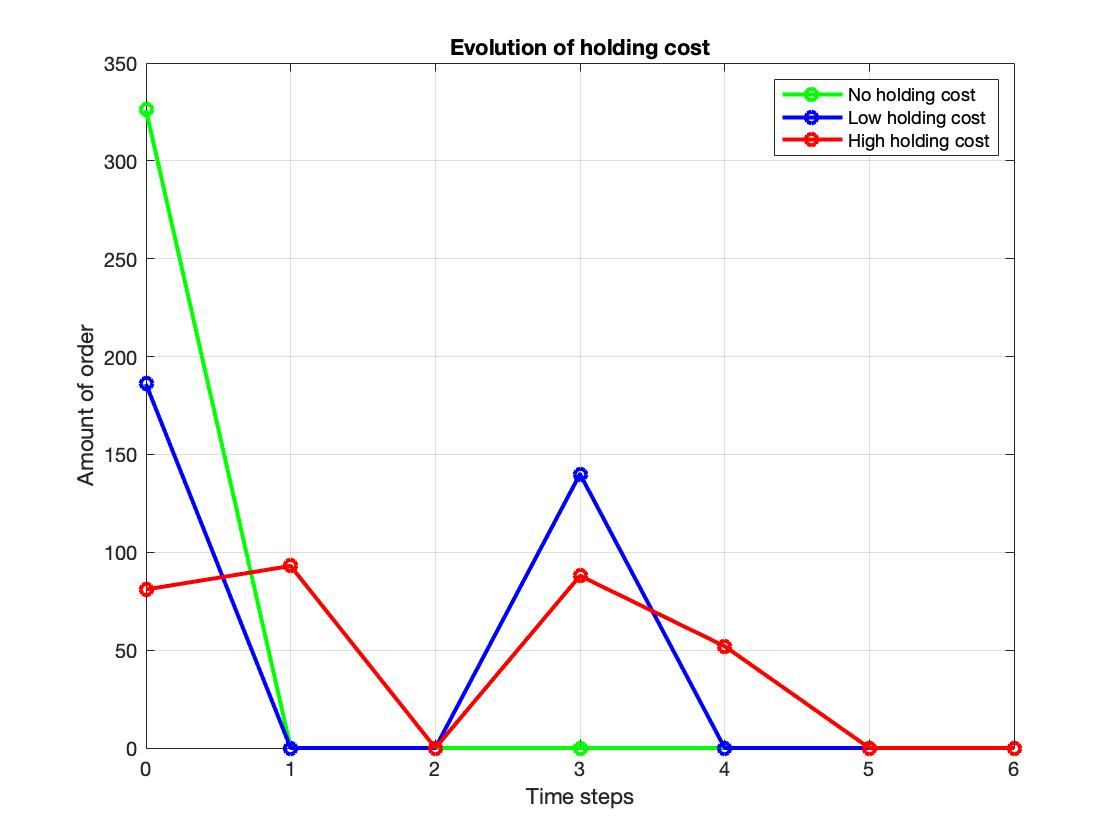
\includegraphics[width=0.7\textwidth]{report-2/fig/holding.jpg}
    \caption{Behaviour of model according to holding cost for product 2}
    \label{fig:holding_cost}
\end{figure}

\begin{table}[H]
    \centering
    \begin{adjustbox}{center}
    \begin{tabular}{|c|c|c|c|c|c|}
    \hline
    & \makecell{\textbf{Holding Cost}\\$[euros]$} & \makecell{\textbf{Extra Cost}\\$[euros]$} & \textbf{Order Evolution} & \makecell{\textbf{Profit} \\$[euros]$} & \textbf{\makecell{Time to \\ Process\\ $[s]$}}\\
    \hline
    \makecell{\textbf{No}\\ \textbf{Holding}} & \makecell{0\\0\\0} & \makecell{0\\0\\0} & \makecell{286\quad0\quad0\quad0\quad0\quad0\quad0\\326\quad0\quad0\quad0\quad0\quad0\quad0\\337\quad0\quad0\quad0\quad0\quad0\quad0} & 18168.04 & 0.448\\
    \hline
    \makecell{\textbf{Low}\\ \textbf{Holding}} & \makecell{1\\1\\2} & \makecell{0\\0\\0} & \makecell{45\quad83\quad14\quad62\quad82\quad0\quad0\\186\quad0\quad0\quad140\quad0\quad0\quad0\\58\quad16\quad85\quad98\quad80\quad0\quad0} & 16540.20 & 2.44\\
    \hline
    \makecell{\textbf{High}\\ \textbf{Holding}} & \makecell{14\\12\\23} & \makecell{0\\0\\0} & \makecell{45\quad61\quad18\quad80\quad82\quad0\quad0\\81\quad93\quad0\quad88\quad52\quad0\quad0\\ 0\quad0\quad0\quad0\quad3\quad0\quad0 } & 3204.30 & 1.22\\
    \hline
    \end{tabular}
    \end{adjustbox}
    \caption{Holding cost analysis with zero extra cost}
    \label{tab:hold_vs_extra}
\end{table}

In "High Holding" section, an other interesting aspect is present: the third product appears to be not convenient to order. In fact, in this simulation the item is characterized by an extremely large holding cost compared to the selling price fixed by the shop owner to 21 euros. This should represent the kind of product complex to maintain and, therefore, inconvenient to be included in the inventory. Even if the system is not interested in buying this product, at time $t=4$ a particularly small amount of 3 items is ordered. Checking the other generated parameters reveals it is not a coincidence, but it is related to discounts. In fact, Supplier 1 offers a 1\% discount in range 9-84 units, but 31\% in range 85-98. The difference is huge. However, at time $t=4$ the system is already ordering 82 units of Product 1 from Supplier 1, so adding 3 units of Product 3 (even if it is a costly product) is a smart choice to get a larger discount on shipping costs. Recalling that the discount is independent by the kind of product, it actually emphasizes the role of optimization: parameters are not stand-alone, but directly linked to compensate costs and exploiting the best strategy.\newline

\noindent
\textbf{Extra costs}\newline
Introducing unsatisfied demand parameters, the situation behaves differently. The model is forced to mitigate this cost. The higher the value, the more the strategy is influenced. 
\noindent
Even if the holding costs and the extra costs are shown together, because they indeed influence each other, their single impact on the simulation is very different.
While the extra costs occur only in case of unsatisfied demand, the holding costs have to be always paid for each item in the inventory. The method is able to adapt better to high extra costs, choosing quantity and timing of orders based on future demand. So, in case of high extra costs, it orders just the amount necessary to fulfill the demand. In case of high holding costs, instead, the method tends to order less items, lowering the quantity of products in the inventory to a strictly necessary level as possible. \par
Table \ref{tab:extra_costs} starts from the "High Holding" case, including some extra costs. Obviously, results and strategies are strongly affected by the values of different parameters. Since extra cost is unitary, its weight is important. In the first case, in fact, also the Product 3 is ordered for the optimal solution. However, the result is negative in terms of profit.
It also re-consider the situation mentioned before of exaggerated holding costs, which are translated in zero orders and profit. If also a large extra cost for unsatisfied demand is implemented, the system is forced to order again to reduce losses, following the evolution of the demand. Otherwise, the model avoids to order, accepting some important losses. Product 3 shows again an elevated holding cost and, despite the extra cost, the ideal solution prevents its order, considering the set parameters of the simulation.

\begin{table}[H]
\vspace{20pt}
    \centering
    \begin{adjustbox}{center}
    \small
    \begin{tabular}{|c|c|c|c|c|c|}
    \hline
    & \makecell{\textbf{Holding Cost}\\$[euros]$} & \makecell{\textbf{Extra Cost}\\$[euros]$} & \textbf{Order Evolution} & \makecell{\textbf{Profit} \\ $[euros]$} & \textbf{\makecell{Time to \\ Process\\ $[s]$}}\\   
    \hline
    
    \makecell{\textbf{High}\\ \textbf{Holding}} & \makecell{14\\12\\23} & \makecell{6\\7\\6} & \makecell{45\quad61\quad18\quad80\quad82\quad0\quad0\\81\quad93\quad12\quad88\quad52\quad0\quad0\\ 58\quad16\quad85\quad98\quad80\quad0\quad0} & -900.06 & 0.73\\
    \hline
    \makecell{\textbf{Exaggerated}\\ \textbf{Holding}} & \makecell{34\\33\\43} & \makecell{23\\25\\22} & \makecell{45\quad61\quad18\quad80\quad82\quad0\quad0\\81\quad93\quad12\quad88\quad52\quad0\quad0\\ 0\quad0\quad0\quad5\quad3\quad0\quad0 } & -26010.08 & 0.722\\
    \hline
    \end{tabular}
    \end{adjustbox}
    \caption{Unsatisfied demand extra cost analysis}
    \label{tab:extra_costs}
\end{table}

Therefore, extra cost should be read as a stimulus to keep ordering, making the system more realistic. In the real world, it will not be just a temporally lack of sales with no gain and no expenses, but a collection of consequences leading the activity out of market. It is remarkable that unsatisfied demand is always present for the first two steps since the initial inventory is set to zero and there is no possibility to meet the demand before the first order arrives (after 2 time steps).
All the instances prove one crucial aspect: the influence of parameters is not absolute. The strategy is not just affected by the presence of a cost, but specially by its magnitude in relation to the others. Even a slight variation in one parameter could lead to a different approach, making less effective other settings. 
\newline
\noindent
\newline
\textbf{Fixed costs}\newline
Keeping the fixed costs fairly low with respect to the unitary costs of items, the algorithm chooses to follow the most convenient pattern, involving different suppliers. On the other hand, if the fixed costs are high, it will tend to order different items from the same supplier. Hence, it obtains an higher discount on the fixed cost, ignoring the larger unitary cost, since holding cost is proportionally lower than the fixed cost without discount.  
Furthermore, in case of really high value of fixed cost, the model performs a large single order at the beginning of the simulation to pay the fixed expense just once, fully exploiting the discount.
This behaviour can be observed in Figure \ref{fig:fix_cost}. The graph is obtained using the same instance, varying only the fixed costs considered equal for all the suppliers.
The figure shows how the model tends to order more items from the same supplier, as the fixed costs get higher. The timing of order distribution is not shown, but the model performs the less orders as possible. It orders an important amount at the starting point of the simulation, preferring the holding costs than paying the fixed cost more than once. This behaviour can be observed in the fixed costs from 4000 to 5000 in the figure: the model in this case orders less items, aggregating the orders. At last, if the fixed costs are equal to 20000, the model performs a single order at the beginning, limiting the provisioning to a supplier only.\par

\begin{figure}[!htb]
    \centering
    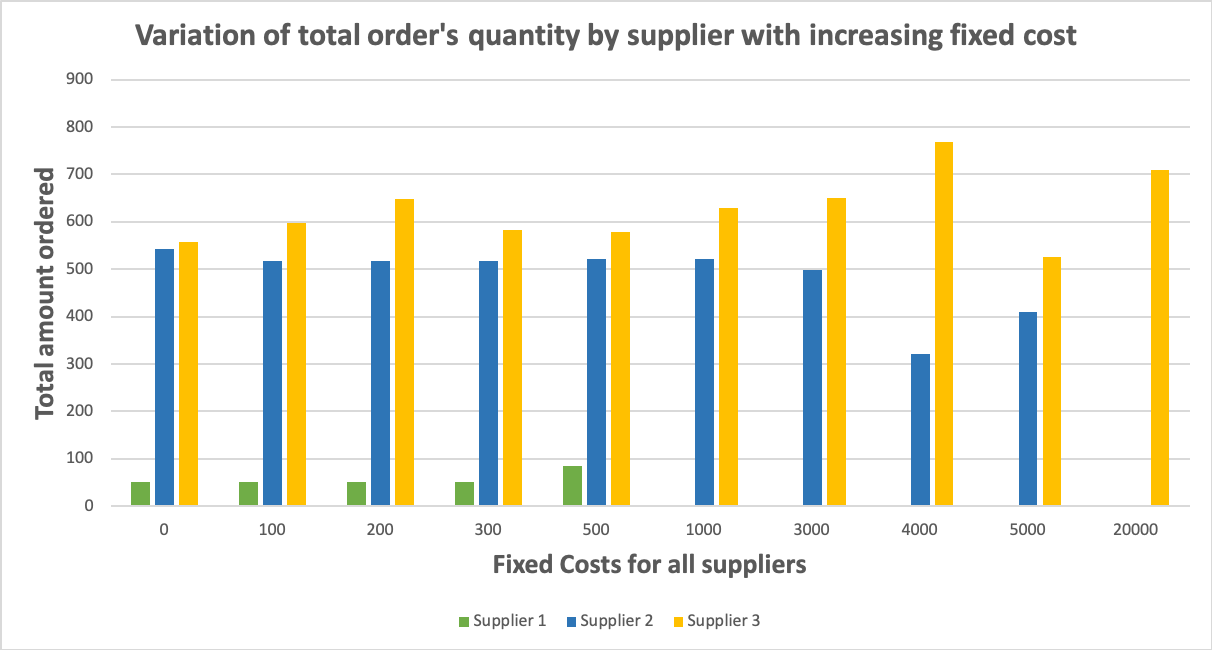
\includegraphics[width=0.9\textwidth]{report-2/fig/fix_cost.png}
    \caption{Orders aggregation with increasing fixed cost}
    \label{fig:fix_cost}
\end{figure}


\noindent
\newline
\textbf{Realistic simulation}\newline
Finally, a complete simulation should be run. A simplified version of instance in Section \ref{sec:instance} is implemented to allow a better reading of results. Peculiar differences are shown in Table \ref{tab:simulation}. The main focus regards the order distribution and choices about the most convenient supplier at each time step, according to the described situation.

\begin{table}[H]
\vspace{30pt}
    \centering
    \begin{subtable}[c]{\textwidth}
        \centering
    \begin{adjustbox}{center}
    \begin{tabular}{|c|c|c|c|c|c|}
    \hline
    & \makecell{\textbf{Initial}\\ \textbf{Inventory}} & \makecell{\textbf{Selling Price}\\$[euros]$} & \makecell{\textbf{Arrival time}\\$[days]$} & \makecell{\textbf{Holding Cost} \\$[euros]$} & \makecell{\textbf{Extra Cost} \\$[euros]$} \\
    \hline
    \textbf{Product 1} & 21 & 26 & 2 & 4 & 9\\
    \hline
    \textbf{Product 2} & 26 & 20 & 2 & 3 & 7\\
    \hline
    \textbf{Product 3} & 23 & 26 & 3 & 4 & 7\\
    \hline
    \end{tabular}
    \end{adjustbox}
    \caption{Shop parameters for inventory}
    \vspace{5mm}
    \end{subtable}
    
    \begin{subtable}[c]{\textwidth}
        \centering
    \begin{tabular}{|c|c|c|c|c|}
    \hline
    & \makecell{\textbf{Fixed Cost}} & \makecell{\textbf{Unitary costs -}\\\textbf{Product 1} \\$[euros]$} & \makecell{\textbf{Unitary costs -}\\\textbf{Product 2} \\$[euros]$} & \makecell{\textbf{Unitary costs -}\\\textbf{Product 3} \\$[euros]$}  \\
    \hline
    \textbf{Supplier 1} & 10 & 5 & NaN & 25  \\
    \hline
    \textbf{Supplier 2} & 500 & 3 & NaN & 4 \\
    \hline
    \textbf{Supplier 3} & 3000 & NaN & 15 & 16 \\
    \hline
    \end{tabular}
    \caption{Suppliers parameters}
    \label{sub:Nan_suppliers}
    \end{subtable}
    \caption{Generic instance for a pseudo-real model }
    \label{tab:simulation}
\end{table}

In particular, in Table \ref{sub:Nan_suppliers}, the "NaN" notation indicates a lack of the product in the specified supplier. This realistic aspect forces the model to consider all the available suppliers in accomplishing the optimal plan. In fact, fixed costs are intentionally unbalanced, distinguishing three distinct levels: low, medium and high. However, discounts and products availability make competitive the apparently inconvenient supplier.
The unitary costs (when present) are always lower than selling prices, but they should not read from an absolute point of view. Every aspect is considered in the relationship with all other parameters, as holding and extra cost, and the potential profit.
Simulation result is shown in Figure \ref{fig:simulation}, with a profit of $6314.2$ \EUR{} and a computation time of $3.31$  seconds. 
\newpage
The graph is particularly interesting: as expected, the system must order (until it is convenient) from the supplier with high fixed cost (green one) to find "Product 2". However, the optimal choice is ordering an important amount at the very beginning only, meeting the demand for the following days. This approach limits the cost, exploiting an high discount.\par
\begin{figure}[!htb]
\vspace{20pt}
    \centering
    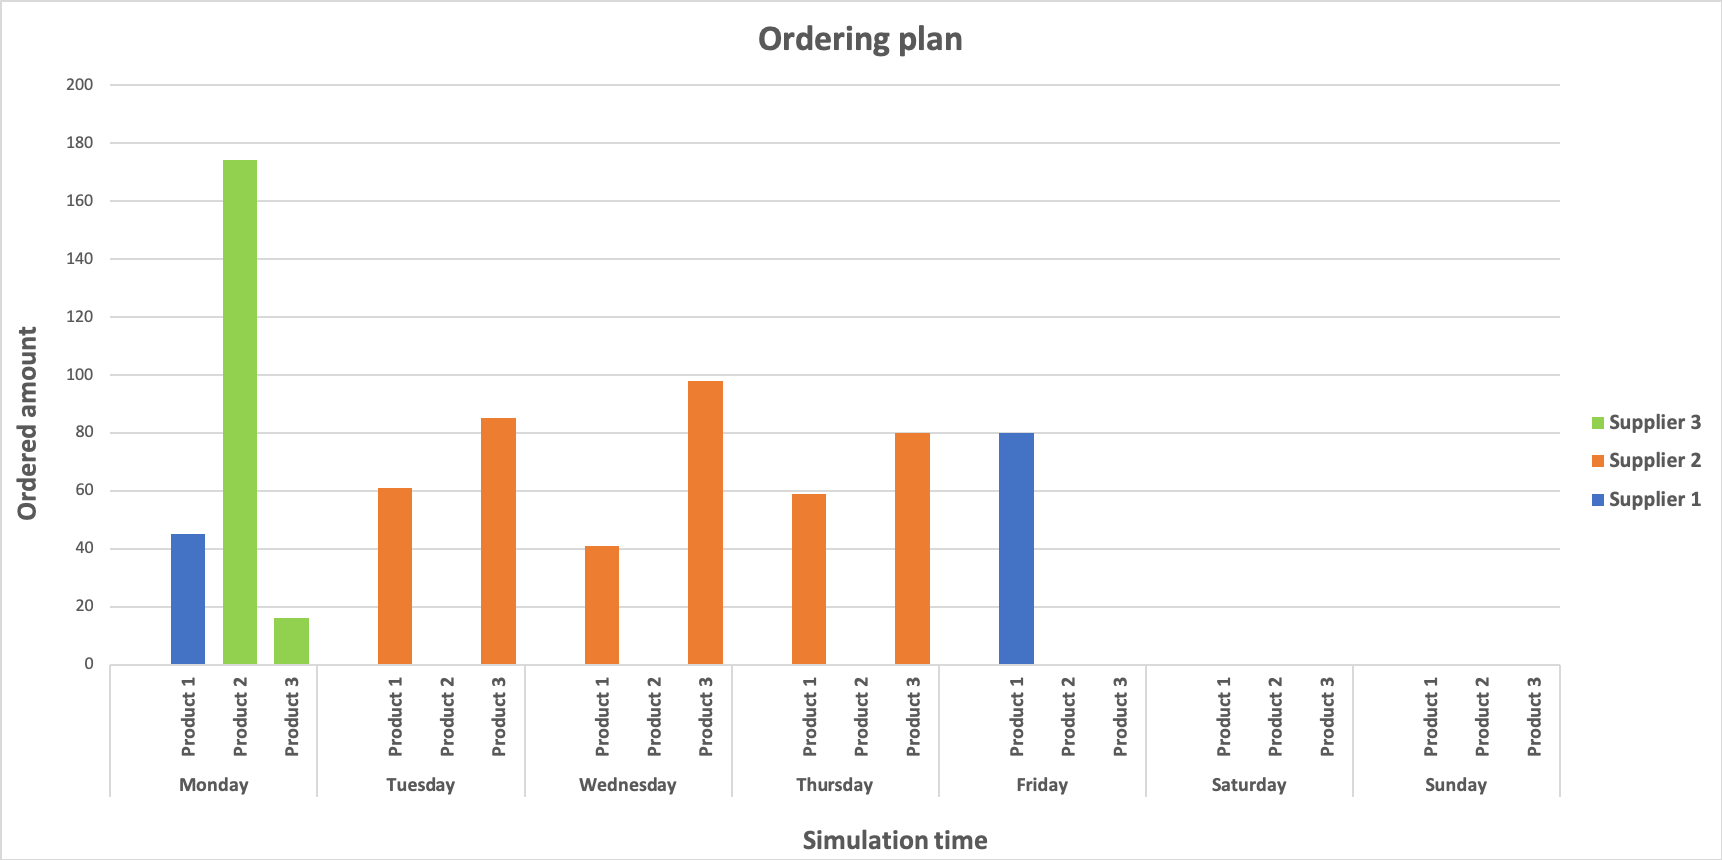
\includegraphics[width=0.9\textwidth]{report-2/fig/Ordering_plan.png}
    \caption{Simulation of ordering plan}
    \label{fig:simulation}
    \vspace{20pt}
\end{figure}
\noindent
"Supplier 2" is instead characterized by the lowest prices on the market for the available products and therefore it is employed more than the others. The reduced fixed cost of "Supplier 1" is not always enough, specially for "Product 3". In fact, the unitary profit would be only the 4\%, without considering all the other costs. 
Concerning the "Product 1", a competition between "Supplier 1" and "Supplier 2" occurs. They present similar unitary cost, but the system prefers the latter whenever it needs "Product 3". Since the connection is opened - and the fixed cost paid - it is more convenient to order also "Product 1", taking advantage of discount. A similar event is observable in Monday, when a small amount of "Product 3" is ordered by "Supplier 3" (despite the unitary cost) since the need of "Product 2". On the other hand, "Supplier 1" is involved only when "Supplier 2" is not. During the last time steps orders are not made since they would not arrive before the end of the simulation.
\newpage

%%%%%%%%%%%%%%%%%%%%%%%%%%%%%%%%%%%%%%%%%%%%%%%%%%%%%%%%%%%%%%%%%%%%%%%%%%%%%
\section{Heuristic}\label{sec:heu}
The approach used for the Heuristic solution is the Greedy Approximate Dynamic Programming. The original model optimizes the profit exploiting the knowledge of the demand for all the time steps of the simulation, while in the Heuristic strategy the profit is optimized time step by time step. This approach is much more simple since, at each time step, the model does not use any estimation of the future demand.\par
The greedy model has to decide whether to order or not based only on the current state of the inventory. An order is made if the amount of product in the inventory is below a given threshold, reducing significantly the solution space of the model. In a realistic scenario, the thresholds should be optimized based on market analysis and past selling records. In this model the thresholds are optimized taking into account inventory and orders of the exact solution. Also, in a realistic scenario, it is more convenient to order less than the demand, especially - as in this case - when no knowledge of the demand at the next time steps is present. This situation is further explored in Section \ref{sec:conclusions}, when the over/under estimation of the demand is analyzed. 

The dynamic programming approach is based on the definition of a set of States and Policies. Given that the exact solution is not a dynamic programming approach, these variables are only related to the heuristic solution. Therefore, they are just valid for the approximate dynamic programming execution.
In this case, the policy is the choice (to order or not) and the possible states are the future possibilities. They should be considered by an exact dynamic programming approach, differently from this implementation. 
As shown in Figure \ref{fig:prob_space_heu}, the probability space related to each single time step is heavily reduced because the algorithm has just two options to consider: to order as much as the demand or not to order at all. 

\begin{figure}[!htb]
\vspace{20pt}
    \centering
    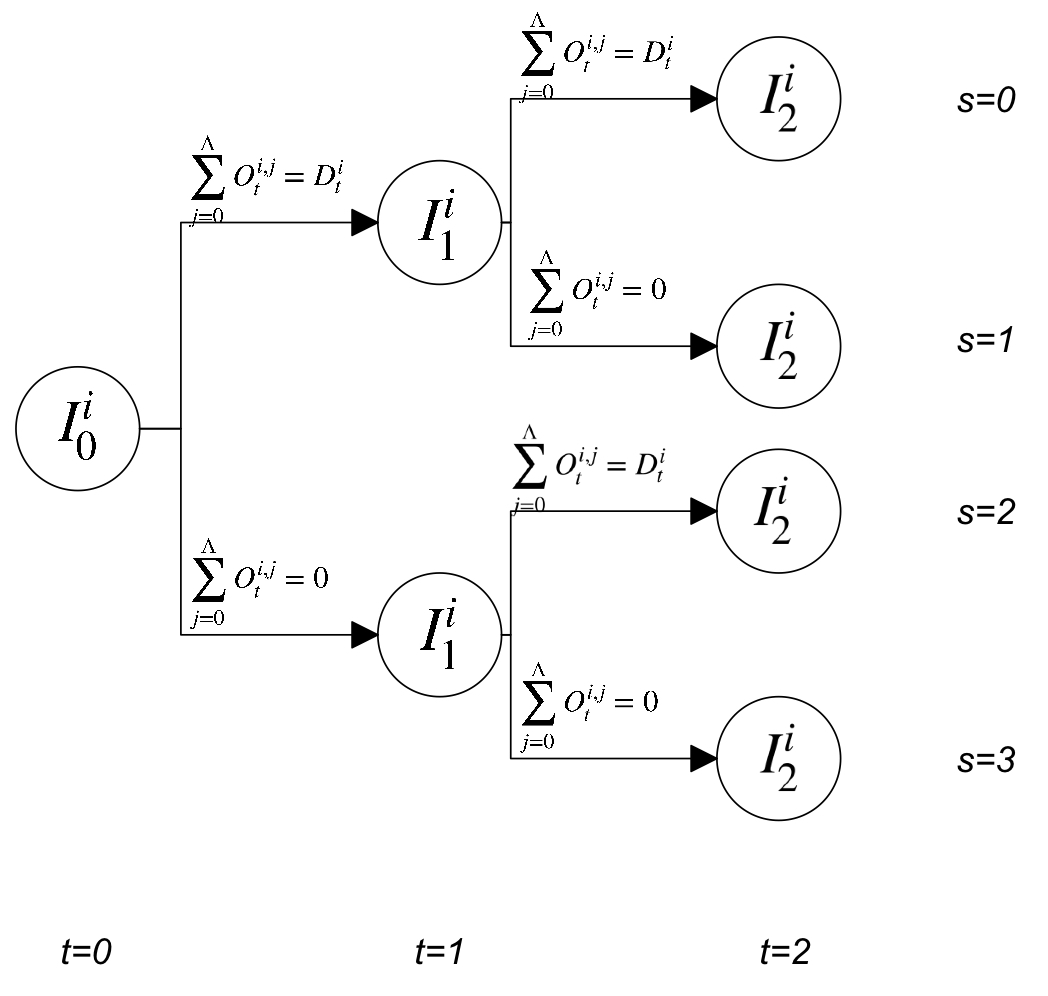
\includegraphics[width=0.7\textwidth]{report-2/fig/prob_space_heu.jpeg}
    \caption{Probability space of Heuristic model}
    \label{fig:prob_space_heu}
\end{figure}

The approximate dynamic programming approach is only applied to the decisions related to the inventory (how much to order and when). It is not used for the decisions regarding the choice of supplier.
The algorithm solves an LP problem equal to the exact one, described in Section \ref{sec:mathModel}, but related to just one time step $t$. The heuristic constraint (\ref{heu_constrain}) is added to the set of constrains. Before starting the optimization, at each time step, the inventory is updated considering the orders made and the items sold in the previous time steps. 

\begin{equation}
   \sum_{j=0}^\Lambda O^{i,j}_t = \begin{cases} 
   D_{t}^i \ \ \ \textit{if} \ \ \ (I_i^{t} < threshold_i) \ \ \textit{and} \ \ (t+T^i < \textit{simulation time period}) \\
   \ \ 0 \ \ \ \ \ \ \ \textit{otherwise} \\
   \end{cases}
   \forall i \in \Theta,  \forall t  \in T\\
   \label{heu_constrain}
\end{equation}
\newline
The variables which determine the performance of the model are the thresholds and the ordered quantity of each item. In the proposed implementation, this quantity is equal to the demand for the item in the time step. Moreover, the exact method avoids to make an order if it will not arrive before the end of the simulation. The same constraint is set also for the heuristic method. In a realistic and unlimited in time scenario, this would be irrelevant. 

\subsection{Computational results}
The performance of the heuristic method depends on the specific instance used for the model. Considering the realistic instance described in Table \ref{tab:description} in Section \ref{sec:instance}, it is evident an improvement in the execution time of the model, despite of a significant profit loss. 
Figure \ref{fig:execution_time} shows that the improvement in the execution time is greater as the number of time steps considered in the simulation gets greater. Each point in the x-axis represents an entire simulation run with that specific number of time steps. The time taken by the exact method to find the solution increases exponentially, while the heuristic method follows a linear growth. In fact, the exact method needs to consider all the possibilities, exploring a much larger probability space. 

\begin{figure}[H]
    \centering
    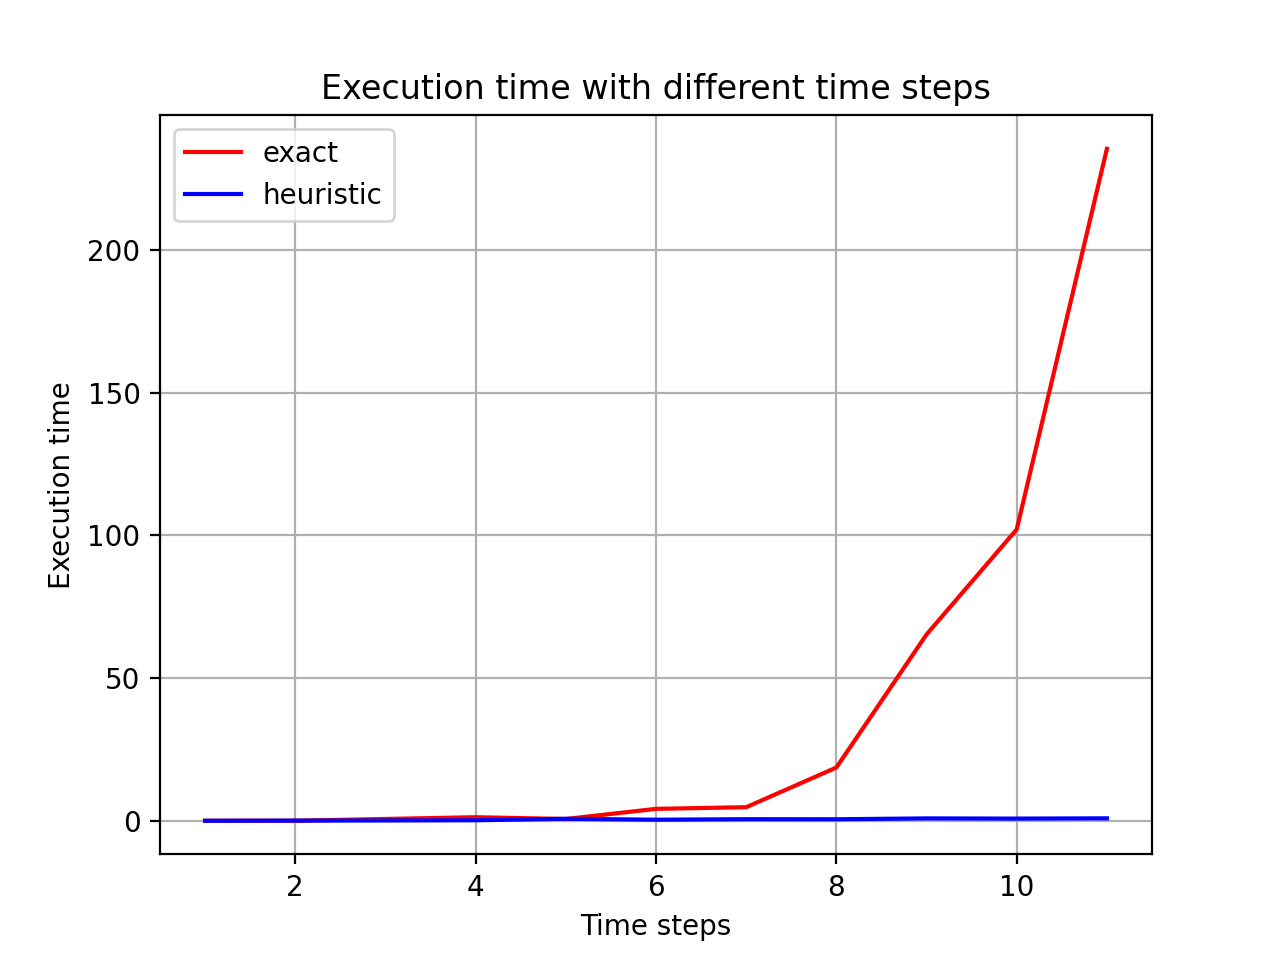
\includegraphics[width=0.8\textwidth]{report-2/fig/ex_time_1_11_1.png}
    \caption{Execution time in milliseconds of simulations as the number of time steps increases}
    \label{fig:execution_time}
\end{figure}

To investigate the heuristic method response to changes in the instance conditions, some simulations have been run in different scenarios. The same thresholds are kept and the results of these simulations are collected in Table \ref{tab:Heur_profit}.
The chosen measure for the performance is the \textit{Percentage profit difference} between the exact and the heuristic profits on the same instance. The profit performance of each simulation has been measured as follows:

\begin{equation}
   \textit{Percentage profit difference} = 100 \  \Bigg|\ \frac{ \textit{Exact profit} - \textit{Heuristic profit} }{\textit{Exact profit}}\ \Bigg | \\ \label{over_prof}
\end{equation}
\newline
Table \ref{tab:Heur_profit} collects the mean and the standard deviation of the \textit{Percentage profit difference} over ten different simulations run with different randomly generated instances. The profit obtained with the realistic instance represents the reference used to evaluate the different scenarios.
\newline
It can be observed that the results are not very far from the optimal ones, at least considering the cases with balanced costs, taking into account the important simplifications introduced. All the results obtained with the different simulations performed in each scenario are represented through the box plot in Figure \ref{fig:box_plot_heu}.

\begin{table}[!htb]
\vspace{15pt}
    \centering
    \captionsetup{justification=centering}
    \begin{tabular}{|c|c|c|}
    \hline
        \textbf{Scenario} & \makecell{\textbf{Average profit} \\ \textbf{difference (percentage)}} & \makecell{\textbf{Standard deviation} \\ \textbf{(percentage)}} \\ \hline 
        \textbf{Realistic scenario} & 23.041 \% & 1.380 \% \\ \hline
        \textbf{Zero pre-orders} & 46.000 \% & 3.906 \% \\ \hline
        \textbf{Arrival time = 1 for all items} & 44.473 \% & 3.255 \% \\ \hline
        \textbf{Very high fixed cost on order} & 110.940 \% & 17.819 \% \\ \hline
        \textbf{Zero Holding costs} & \multirow{2}{*}{14.022 \%} & \multirow{2}{*}{1.051 \%} \\ 
        \textbf{Zero Extra costs} & & \\\hline
        \textbf{Very high Holding costs} & \multirow{2}{*}{46.232 \%} & \multirow{2}{*}{0.533 \%} \\ 
        \textbf{Zero Extra costs} & & \\\hline
        \textbf{Zero Holding costs} & \multirow{2}{*}{122.672 \%} & \multirow{2}{*}{2.779 \%} \\ 
        \textbf{Very high Extra costs} & & \\\hline
    \end{tabular}
    \caption{Profit comparison between Heuristic and Exact solution in different scenarios \\(over 10 measures with different instances)}
    \label{tab:Heur_profit}
    \vspace{20pt}
\end{table}
\begin{figure}[!htb]
    \centering
    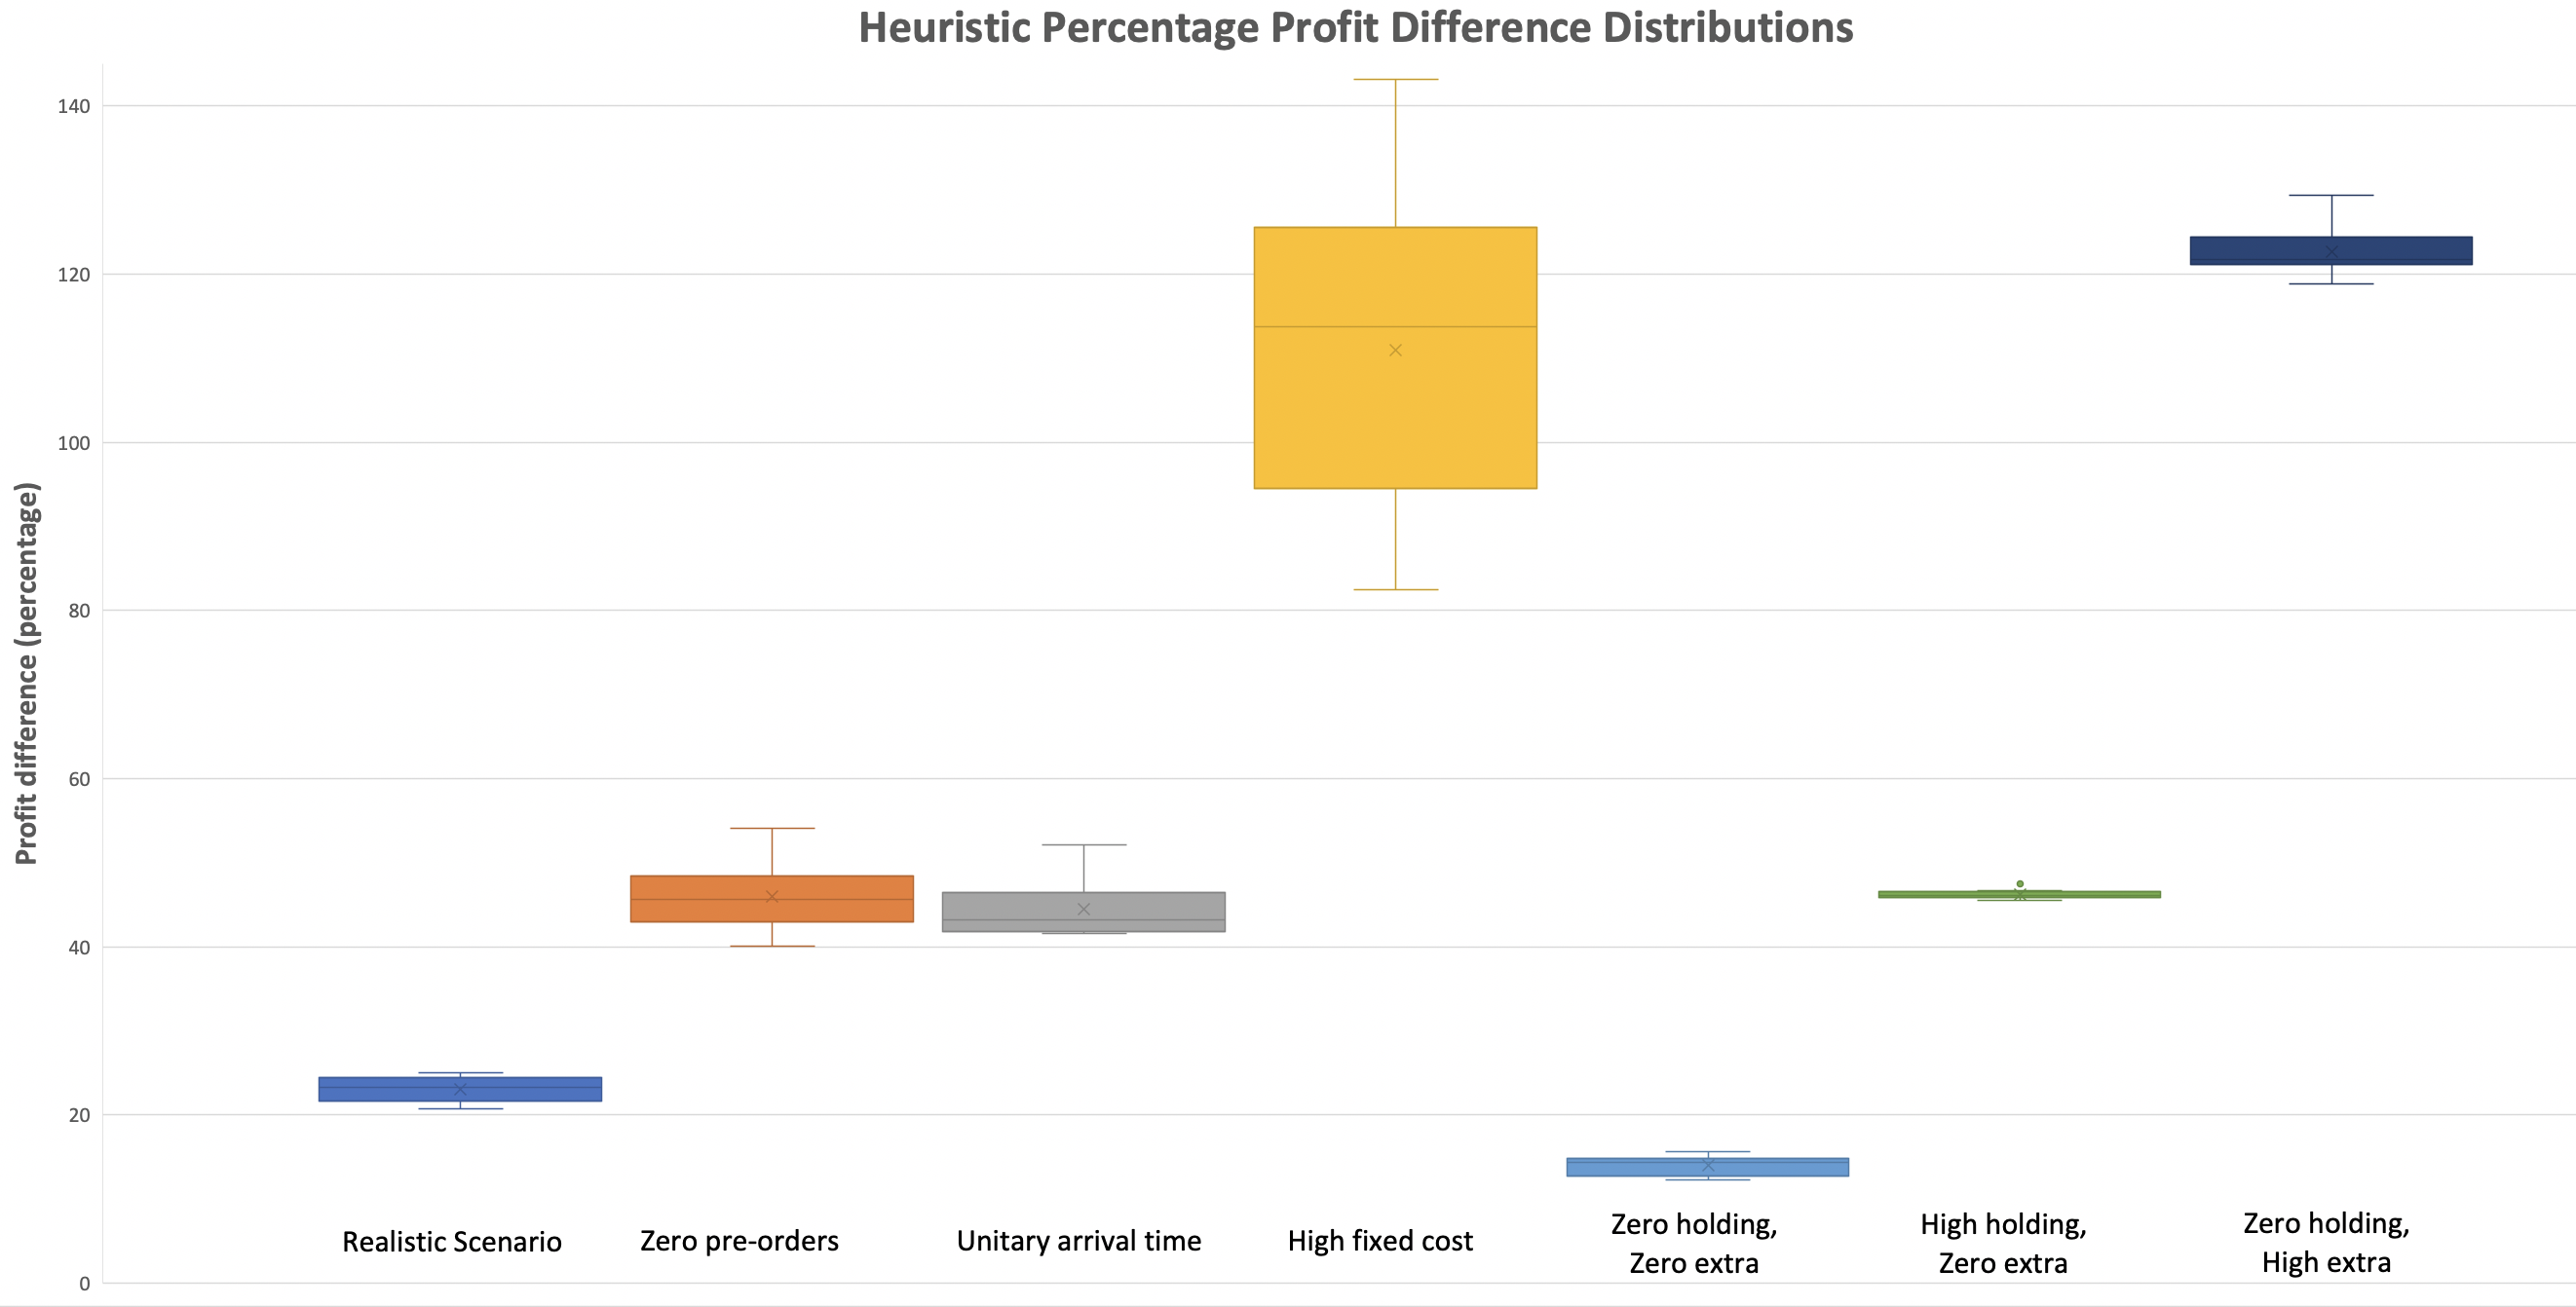
\includegraphics[width=0.95\linewidth]{report-2/fig/box_plot_heu.png}
    \caption{Box Plot of profit difference between Heuristic and Exact solution}
    \label{fig:box_plot_heu}
    \vspace{15pt}
\end{figure}

The case with zero pre-orders is unsatisfactory for both methods, because pre-orders introduce items in the inventory without the need to pay for them in the simulation time. The difference in profit is greater than the realistic instance because of their absence. Therefore, both methods are forced to make more orders in the first time steps. 
\newline
\noindent
Since the ones made by the exact method are better optimized, the resulting profit is higher. Moreover, the thresholds of the heuristic are set according to the result of the optimal method with pre-orders, so they are less suited to this situation. The same problems occur also in the case with arrival time of all the items set to 1. In this condition, the thresholds cause more critical issues. In fact, the exact method plans smaller and more frequent orders, differently from the policy used in the realistic scenario (up to 5 time steps). 
This heuristic implementation is not time-aware and this is one of the main weaknesses. It is particularly noticeable in the instance with very large fixed costs. The same situation was also analyzed in Section \ref{subsec:computational_results_exact} for the exact method. The heuristic could not behave like in Figure \ref{fig:fix_cost} because it is not able to aggregate orders in time. 
\newpage \noindent
To verify, the fixed costs are set to 20000 for all suppliers (value for which the exact model aggregates all of the orders in one time step, from one supplier only).
The heuristic orders exactly the same amount as the other simulations, since it can just choose the supplier to order from. \par

The heuristic method is also vulnerable to the case of high extra-costs, due to the lack of adaptability. In fact, it presents no capacity to decide the amount to order for any items. The system simply orders as much as the demand of the current moment (no knowledge of future demand). 
The situation is different in case of high holding costs. Both exact and heuristic solutions are less robust. The latter is even less adaptable, considering that holding costs are compulsory, while extra costs appear only in case of unsatisfied demand. \par

An interesting result is obtained applying the soft policies technique, as described by \cite{Cimen2013}. This approach is based on the definition of an exploration/exploitation rate. The main idea is that the best choice could not be the Greedy one in some cases. So, the model can make a different decision according to the value of the mentioned rate. In this specific implementation, the rate is defined as a value $\epsilon$ between 0 and 1, which represents the probability that the model will not respect the constraint (\ref{heu_constrain}), making the opposite choice (not order if the inventory is below the threshold and vice versa). Applying this condition, the right choice of $\epsilon$ leads to a small improvement in the profit performance of the heuristic method, listed in Table \ref{tab:epsilon}.

\begin{table}[!htb]
    \centering
    \vspace{20pt}
    \begin{tabular}{|c|c|c|c|}
    \hline
        \makecell{\textbf{Epsilon ($\epsilon$)}} & \makecell{\textbf{Average profit} \\ \textbf{difference (percentage)}} & \makecell{\textbf{Standard deviation} \\ \textbf{(percentage)}} & \makecell{\textbf{Opposite decision}}\\ \hline
        \textbf{0} & 23.041 \% & 1.380 \% & 0\\ \hline
        \textbf{0.03} & 20.587 \% & 0.729 \% & 3\\ \hline
        \textbf{0.05} & 20.659 \% & 0.731 \% & 4\\ \hline
        \textbf{0.1} & 20.679 \% & 1.098 \% & 6\\ \hline
        \textbf{0.2} & 23.441 \% & 2.358 \% & 8\\ \hline
        \textbf{0.25} & 32.341 \% & 3.021 \% & 11\\ \hline
    \end{tabular}
    \caption{Profits with different values of exploration/exploitation rate}
    \label{tab:epsilon}
    \vspace{20pt}
\end{table}

Obviously, an exaggerated high value of $\epsilon$ introduces important randomness into the solution, causing low profits. The "Opposite decisions" column represents the number of times the model takes the opposite decision due to a random extraction. The most convenient solution is obtained setting $\epsilon = 0.03$, which corresponds to three opposite decisions.\par
Pondering all these considerations, the heuristic method is clearly dependent on the parameters used to optimize it. It is not flexible and suited for important variations in the instance of the problem. In a more reliable scenario, realistic data should be used to set parameters, assuming a predictable behavior of the whole system. The heuristics solution could be significantly improved, in terms of profit, implementing a partially time-aware system, taking into account the demand of a limited number of periods. 
Overall, if the initial condition remains similar, this heuristic implementation provides a satisfying profit result, more time-efficient with respect to the exact one. 
\newpage

%%%%%%%%%%%%%%%%%%%%%%%%%%%%%%%%%%%%%%%%%%%%%%%%%%%%%%%%%%%%%%%%%%%%%%%%%%%%%
\section{Discussion and Conclusions}\label{sec:conclusions}
The values of the demand used to perform the simulation could represent the results of an estimation made by the shop owner for the next time period (in this case, the seven days ahead). To evaluate the influence of an over/under estimation of the demand, the optimal parameters obtained from the simulation of the exact model are applied to a new scenario, in which the demand is incremented or decremented by a constant value. The  achieved profits under these modified conditions are then compared to the ones got from the original simulation. The results are reported in the graph in Figure \ref{fig:overDemand}.
\begin{figure}[!htb]
    \centering
    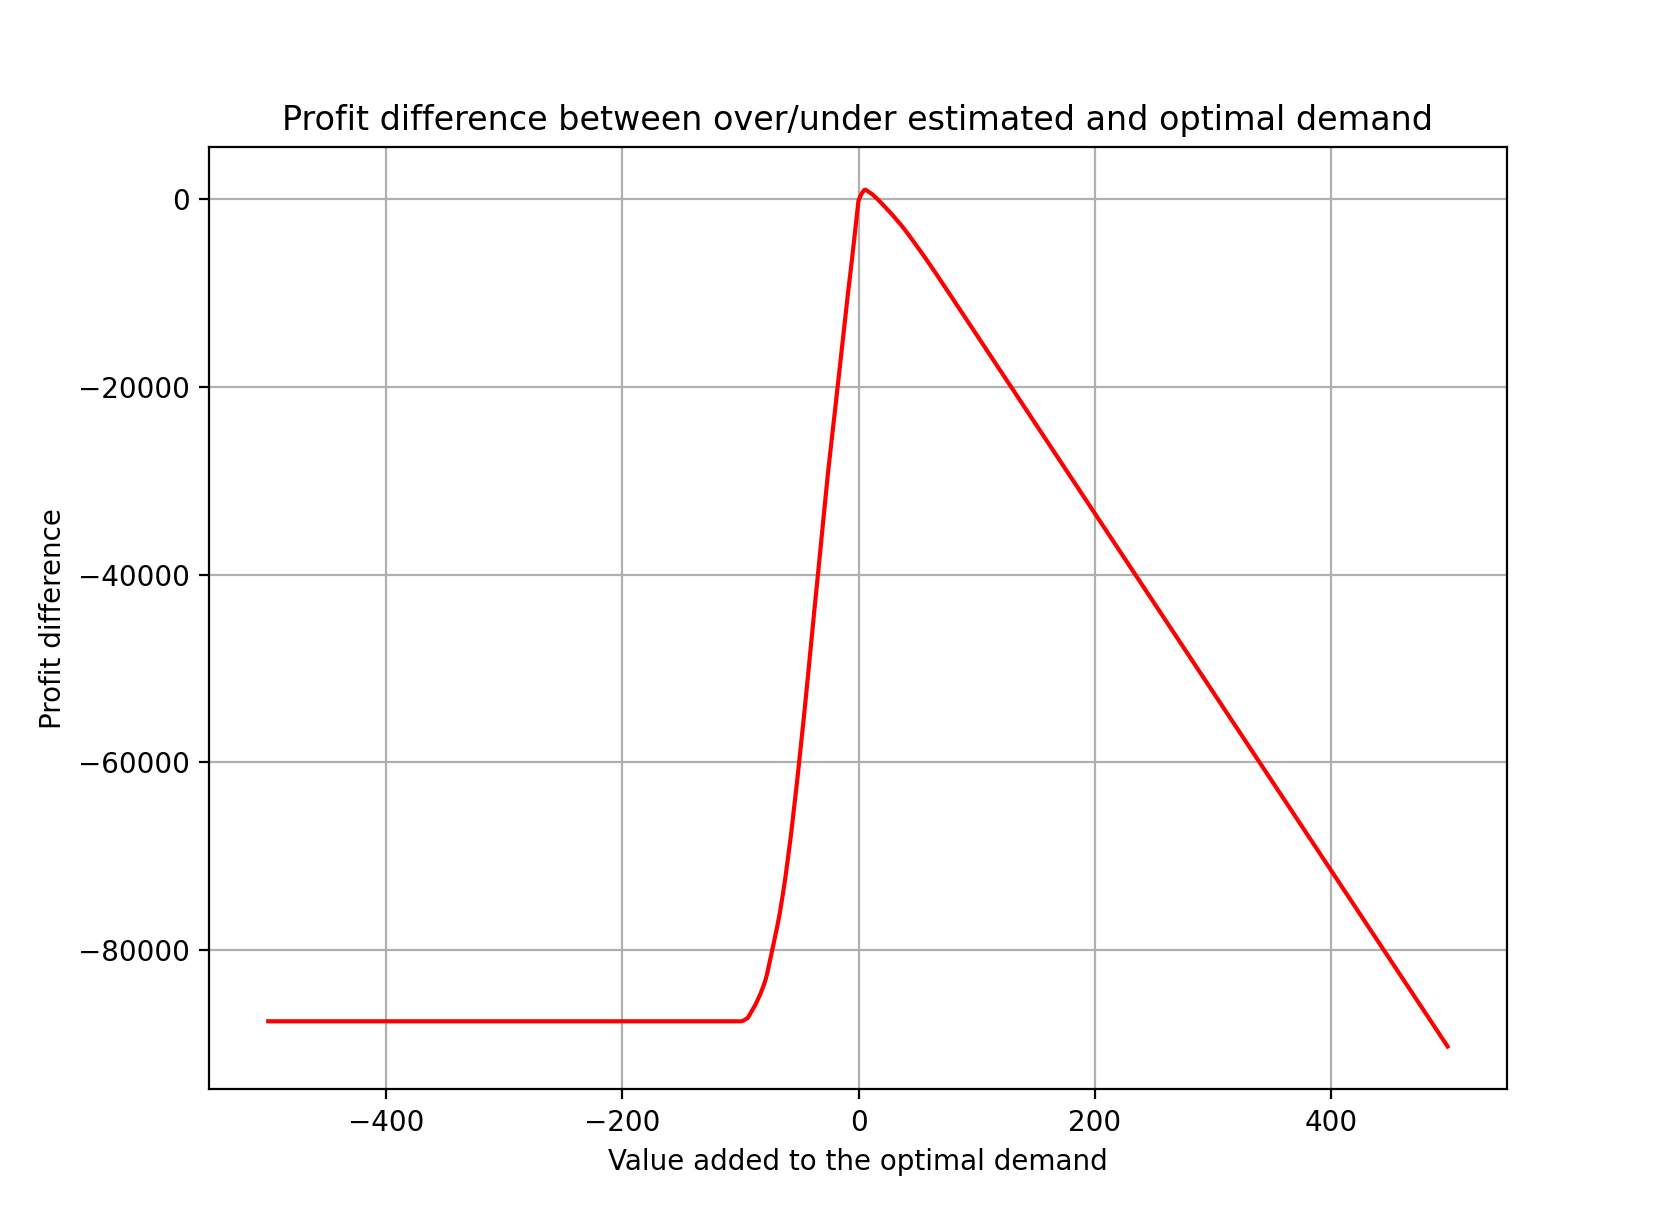
\includegraphics[width=0.8\textwidth]{report-2/fig/overDemand.png}
    \caption{Profit difference between over/under estimated and optional demand}
    \label{fig:overDemand}
\end{figure}\\
The x-axis represents the variation of the optimal demand, increased or decreased to stress the over/under estimation. Instead, on the y-axis the respective profit difference is shown. These values are obtained by subtracting the optimal profit from the over/under estimated ones as shown in Equation (\ref{over_prof_eq}). 
\begin{equation}
   \textit{Profit difference} = \textit{Profit due to over/under estimation} - \textit{Optimal Profit} \\ \label{over_prof_eq}
\end{equation}
Clearly, the profit decreases both on the right and on the left side of the zero value, which represents the optimal demand condition. In particular, for an increasing under estimation of the demand (right side of the graph) the profit decrease is slower with respect to the fast drop obtained in the left side (over estimation growth). In fact, with an under estimated demand, all the earnings obtained by sales remain unchanged. 
The only extra expense is due to the unsatisfied demand costs. On the other hand, with an over estimated demand, the amount of items sold - and the consequent earning - is lower compared to the optimal condition. Furthermore, the holding costs for the unsold items have to be paid. \par 
The curve in the graph, in addition, is flat for values of the extra demand below $-100$. This behaviour is due to the imposed condition for which the amount of products in the inventory must not be below the zero. \par 
Results are obtained using the values of instance in Table \ref{tab:description} in Section \ref{sec:instance} which represents a generic realistic scenario. In these conditions - and given all the considerations made in the paragraphs above - it is better to under estimate than to over estimate the demand by the same amount. This result can be interesting also from an ecological point of view: for certain items, fewer orders could reduce the waste of products. Especially in a circular economy perspective, higher accuracy could be achieved including considerations about the economic and environmental costs, related to the waste disposal of the product and its trend to be unsold. 
\newpage This is inevitably dependent on the type of product. In any case, different kinds can be involved, from perishable goods - like food - to fast-obsolescing items as clothes or technological products, which get easily replaced by newer and more sophisticated versions. 
 \par
As seen from the obtained results, the model itself is strongly dependent on the estimation of the demand, the actual core of the strategy. Although that aspect is beyond the purpose of this paper, it could be interesting to explore different strategies for a better estimation of the demand. The most common approach concerns market analysis and selling records. A more modern technique could also involve big data analysis using machine learning on a broader range of variables, such as weather conditions or geopolitical and social factors. 
\par
Remarking that selling prices are parameters and not a decision variable, they are fundamental in the ordering strategy. In fact, costs should be minimized compared to earnings of the shop. However, the optimal solution is not always directly linked to the specific earning of each item. Choices are made to maximize the total profit, seen by a more general perspective. Each item presents its set of costs, uncorrelated from the others. On the other hand, since orders are packed to manage fixed costs and to take advantage of suppliers discounts, the approach should not consider products separately only. Nevertheless, in the general trade-off, some items could result inconvenient to order according to their costs and their demand.
\par

In this paper, inventory optimization is described, including the selection of the optimal supplier to order from. As mentioned before, the mathematical model can be an important starting point for many different applications, including \textit{ad hoc} parameters to build more suitable scenarios. In the appropriate environment, a special focus should be reserved to the improvement of the Heuristic solution in order to be efficient (also in complex conditions) reducing the profit difference from the exact one.
\newpage

\bibliography{mybibfile}
\end{document}